\documentclass[b5paper,10pt]{article}
\usepackage[colorlinks=true,linkcolor=blue]{hyperref}
\usepackage{graphicx}
\usepackage{tikz-cd}
\usepackage{notestemplate}
\usepackage{mathtools}
%\usepackage[screen]{pdfscreen}
\DeclarePairedDelimiter{\abs}{\lvert}{\rvert}
\usepackage{fontspec}
\usepackage{cite}
%\setmainfont{Times New Roman}
\title{Motivic Homotopy Theory}
\author{Chow.}
\date{}
\begin{document}
\maketitle
\begin{center}
	
\includegraphics[height=4cm]{PIC/xiaohui.eps}
\end{center}
\tableofcontents
	\section{Unstable Homotopy Category}
	In order to refine the triangulated category of Voevodsky's motives and apply more tools from algebraic topology, we need well-behaved homotopy theory for schemes. Homotopy theory for schemes also allow us to construct motivic cohomology and algebraic K-theory which are looked as generalized cohomology theory defined with Brown representativity theorem.
	\subsection{Simplicial Methods for Algebraic Geometry}
	Let us firstly recall some simplicial homotopy theory.
	$\Delta$ is category consists of objects such as
	\[
	[n]={0 \to 1 \to 2 \to \cdots \to n}
	\]
	for all non-negative integer $n$. And morphisms are functions of sets preserving the order of arrows.
	The category of \emph{simplicial sets} means the category of presheaves on $\Delta$ with values over $\mathbf{Sets}$. It is denoted by $\mathbf{sSets}$.
	
	In category of simplicial sets, we have following canonical objects
	\[
	\Delta[n] := \Delta(-,[n])
	\]
	They are call \emph{standard simplicial sets}.
	\begin{secprop}
		$\Delta([m],[n])$ is generated by following morphisms
		\[
		\begin{aligned}
			d^i \colon [k] &\to [k+1]\\
			d^i(0 \to 1 \to 2 \to \cdots \to k)&=\begin{cases}
			1\to 2 \to \cdots \to k+1& \text{if } i =0\\
			0 \to 1 \to \cdots \to i-1 \to i+1 \to \cdots \to k+1& \text{if } 1\leq i \leq k\\
			0 \to 1 \to \cdots \to k& \text{if } i =k+1\\
			\end{cases}
		\end{aligned} 
		\]
		and
		\[
		\begin{aligned}
		s^i \colon [k] &\to [k-1]\\
		s^i(0 \to 1 \to 2 \to \cdots \to k)&=\begin{cases}
		0\to 0 \to 1 \to \cdots \to k-1& \text{if } i =0\\
		0 \to \cdots \to i \to i  \to \cdots \to k-1& \text{if } 1\leq i \leq k-1\\
		\end{cases}
		\end{aligned} 
		\]
		where $d^i$ is called co-face map and $s^i$ is called co-degeneracy map.
	\end{secprop}
$\Delta$ is small category. As diagram, $\Delta$ looks like
\[
\begin{tikzcd} 
 {[0]} \arrow[r, shift left,"d^0"] \arrow[r, shift right,"d^1"'] & {[1]} \arrow[r,"d^0" description] \arrow[r, shift left=4,"d^1"] \arrow[r, shift right=4,"d^2"'] & \cdots 
\end{tikzcd}
\]
\[
\begin{tikzcd} 
{[0]} \arrow[r,"s^0",leftarrow] & {[1]} \arrow[r,shift left,"s^0",leftarrow] \arrow[r, shift right,"s^1"',leftarrow]  & \cdots 
\end{tikzcd}
\]
By Yoneda lemma, for simplicial set $X \in \mathbf{sSets}$, we have 
\[
X([n])\simeq \mathbf{sSets}(\Delta[n], X)
\]
For convenience, we always denote $X([n])$ by $X_n$ for simplicial set $X$, $d_i = X(d^i)$ and $s_i= X(s^i$). 
\begin{figure}[h]
	\caption{Idea of simplicial sets (from ncatlab)}
\centering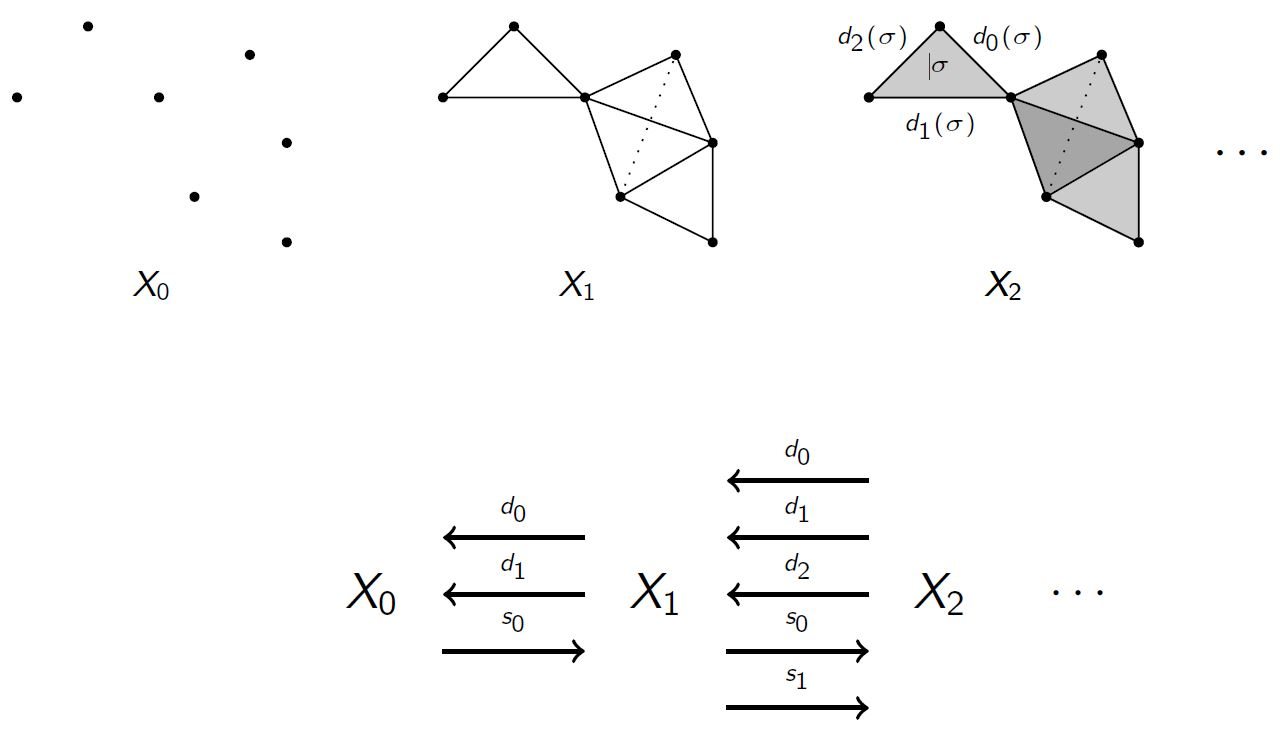
\includegraphics[scale=0.5]{PIC/SimplicialSetsIdea.jpg}
\end{figure}

Let $\Delta^n$ be standard simplex in topological space category. Then we can defined topological space respect to given simplicial set $X$ as follows
\[
|X| := \colim_{(\Delta_n \to X) \in \mathbf{sSets}/X} \Delta^n
\]
Furthermore, $|-|$ is covariant functorial in $\mathbf{sSets}$ since co-representable $\mathbf{sSets}(\Delta_n,-)$ and colimit are functorial. $|-|$ is called \emph{geometric realization functor}.
For standard simplicial set $\Delta[n]$, we can define $k$-\emph{horn} as
\[
\Lambda^k[n] = \bigcup_{i \neq k} \partial^i \Delta[n]
\]
For example, $\abs{\Lambda^0[2]}$ looks like
\begin{figure}[h]
	\centering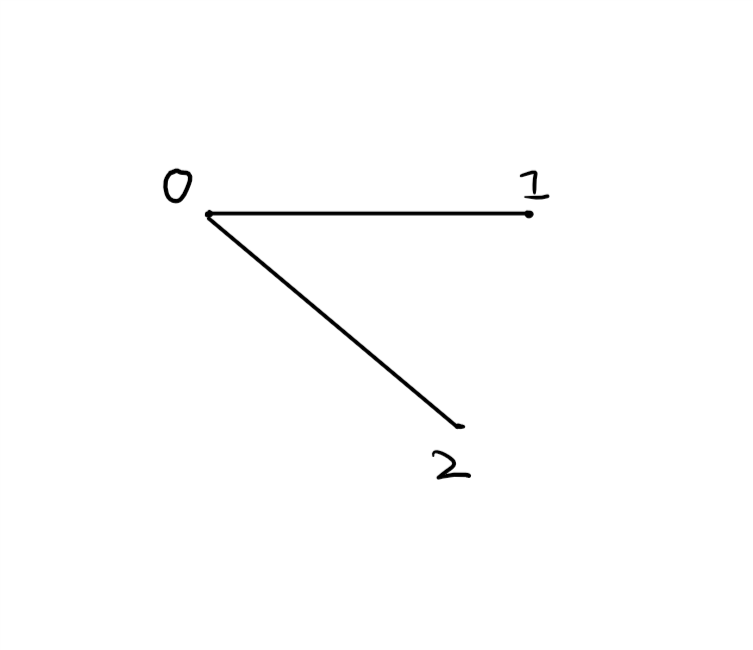
\includegraphics[height=0.15\textheight ]{PIC/horn.png}
\end{figure}
\begin{secdefn}
	The morphism $f \colon X \to Y$ between simplicial sets is called Kan fibration if in square
	\[
	\begin{tikzcd}
	&\Lambda^k[n] \ar[r] \ar[d,hook]& X \ar[d,"f"]\\
	& \Delta[n] \ar[r] & Y \\
	\end{tikzcd}
	\]
	the lifting from $\Delta[n]$ to $X$ exists, where $\Lambda^k[n] \hookrightarrow \Delta[n]$ is the natural inclusion of horn.
\end{secdefn}
In classical simplicial homotopy theory, we can endow $\mathbf{sSets}$ with model structure where fibrations are Kan fibrations and weak equivalence are morphisms which induce isomorphisms between fibrant objects on homotopy groups (can be defined as homotopy groups of corresponding geometric realizations).
\subsubsection{Simplicial Objects}
Let $\mathcal{C}$ be arbitrary (concrete) category. We say $X_*$ is a \emph{simplicial object} on $\mathcal{C}$ if $X_*$ is a presheaf $X_* \colon \Delta^{op} \to \mathcal{C}$ and $\mathbf{s}\mathcal{C}$ denotes the category of simplicial objects on $\mathcal{C}$. Hence simplicial sets are simplicial objects on $\mathbf{Sets}$. 

Let $\Delta_{\leq n}$ the full subcategory of $\Delta$ generated by objects $\{0,1, \cdots, n \}$ and $s_n \mathcal{C}$ the category of presheaves of objects in $\mathcal{C}$ on $\Delta_{\leq n}$, these objects are called $n$-truncated simplicial objects in $\mathcal{C}$. Composite with inclusion $\Delta_{\leq n} \hookrightarrow \Delta$, we get functor
\[
(-)_{\leq n} \colon s\mathcal{C} \to s_n \mathcal{C}
\]
. It is called $n$-truncation functor. It has right adjoint functor 
\[
\begin{tikzcd}
(-)_{\leq n} \colon s\mathcal{C} \ar[r, shift left = 1] \ar[r, leftarrow, shift right =1]& s_n \mathcal{C}\ :\cosk_n
\end{tikzcd}
\]
and left adjoint functor 
\[
\begin{tikzcd}
\sk_n \colon s_n\mathcal{C} \arrow[r, shift left =1] \arrow[r, leftarrow, shift right=1]& s\mathcal{C}\ : (-)_{\leq n}
\end{tikzcd}
\]
More concretely, $\sk_n(X_{\leq n})$ is smallest subobject of $X$ in $s\mathcal{C}$ agrees with $X$ in dimension lower than $n$ and $\cosk_n(X_{\leq n})_k$ is $\mathcal{H}om(\sk_n(\Delta([k])_{\leq n}),X) $ for all $k$.

If $\mathcal{A}$ is  an Abelian category, then we have following correspondence
\begin{secprop}[Dold-Kan Correspondence]
\[
N \colon s\mathcal{A} \to \mathbf{Ch}_{\geq 0} (\mathcal{A})
\]
is equivalence of categories and is also Quillen equivalence (i.e.\ Quillen functor induce equivalence between homotopy categories) with respect to canonical model structure on $s\mathcal{A}$ and projective model on $\mathbf{Ch}_{\geq 0 } (\mathcal{A})$. $N$ is functor of normalized complex and $\mathbf{Ch}_{\geq 0}(\mathcal{A})$ is category of non-negative chain complexes. This equivalence is called \emph{Dold-Kan correspondence}.
\end{secprop}
This proposition means that homological algebra over Abelian category in low bounded case is equivalent to homotopy theory for its simplicial objects. It is convenient to study homotopy theory for simplicial objects because we have geometric realization functor to make constructions more natural. So we can transplant properties from classical homotopy theory into homological algebra.
\subsubsection{Simplicial Homotopy Theory for Presheaves and Sheafification}
Suppose $\mathbf{PSh}^{\mathbf{Sets}}(\mathcal{C})$ be the category of presheaves of sets on $\mathcal{C}$. Then the associated category of simplicial objects $s\mathbf{PSh^{Sets}}(\mathcal{C})$ is isomorphic to $\mathbf{PSh^{sSets}}(\mathcal{C})$ --- the category of presheaves of simplicial sets on $\mathcal{C}$. Let $X_* \in s\mathbf{PSh^{Sets}}(\mathcal{C})$
\[
F_* \mapsto F
\]
where \[
F(X)_n := F_n(X) \ \forall X \in \mathcal{C}
\]
In this case, $s\mathbf{PSh^{Sets}}(\mathcal{C})$ or $\mathbf{PSh^{sSets}}(\mathcal{C})$ is called category of simplicial presheaves of sets on $\mathcal{C}$.

$\mathbf{PSh^{sSets}}(\mathcal{C})$ can be endowed with model structure objectwise by model structure of $\mathbf{sSets}$.
\begin{itemize}
	\item $\alpha \colon F \Rightarrow G$ is weak-equivalence if and only if for all $X \in \mathcal{C}$, $\alpha_X: F(X) \to G(X)$ is weak-equivalence in $\mathbf{sSets}$.
	\item $\beta\colon F \Rightarrow G$ is fibration if and only if for all $X \in \mathcal{C}$, $\beta_X$ is Kan fibration.
\end{itemize}
Then the model structure of $\mathbf{PSh^{sSets}}(\mathcal{C})$ is fibrantly generated. This model structure on $\mathbf{PSh^{sSets}}(\mathcal{C})$ is called \emph{global model structure}.

If $\mathcal{C}$ is a site with Grothendieck topology, we can define $\mathbf{Sh^{sSets}_\tau} (\mathcal{C})$ be the category of $\tau$-sheaves of sets on $\mathcal{C}$ and $\mathbf{PSh_\tau^{sSets}}(\mathcal{C})$ the category of simplicial presheaves with model structure called \emph{$\tau$-local model structure} as follows. 
\begin{secdefn}[$\tau$-local weak equivalence]
	A \emph{$\tau$-local weak equivalence} is a morphism between presheaves $f \colon F \Rightarrow G$ such that
	\begin{itemize}
		\item The morphism induces isomorphism $\tilde{\pi}_0(f): \tilde{\pi}_0X \to \tilde{\pi}_0Y$ in $\mathbf{Sh^{Sets}}(\mathcal{C})$;
		\item For all $U \in \mathcal{C}$, $\tilde{\pi}_n(f): \tilde{\pi}_n(X,x) \to \tilde{\pi}_n(Y,f(x))$ is isomorphism on $\mathcal{C}/U$ for any choice of base point $x \in X(U)$.
	\end{itemize}
\end{secdefn}
The $\tau$-local cofibrations are same as ordinary cofibrations of $\mathbf{PSh^{sSets}}(\mathcal{C})$ and $\tau$-fibrations are morphisms in $\mathbf{PSh^{sSets}}(\mathcal{C})$ satisfy RLP for $\tau$-acyclic cofibration (i.e.\ be both $\tau$-cofibration and $\tau$-weak equivalence). Jardine proved that these datum actually define a model structure.

In particular, if $\mathcal{C}=(Sm/S)_\tau$ is site of smooth $S$-schemes with Grothendieck topology $\tau$, we denote $\mathbf{Spc}^{pre}(S)$ (resp.\ $\mathbf{Spc}_\tau^{pre}(S)$, resp.\ $\mathbf{Spc}_\tau(S)$) the category of simplicial presheaves (res.\ simplical presheaves with $\tau$-local model structue, resp.\ simplicial $\tau$-sheaves) on $\mathcal{C}=(Sm/S)_\tau$. $\mathbf{Spc_\tau}(S)$ is full subcategory of $\mathbf{Spc}^{pre}_\tau(S)$ and left adjoint functor $s$ of inclusion exists. This fucntor is called is called \emph{sheafification functor} under topology $\tau$. Hence $\mathbf{Spc_\tau}(S)$ is model category. Furthermore, we have 
\begin{secprop}
	The pair $(s ,i)$ of adjunction is a pair of Quillen equivalence.
\end{secprop}
Hence we have $\mathbf{Ho}(\mathbf{Spc}_\tau^{pre}(S)) \simeq \mathbf{Ho}(\mathbf{Spc}_\tau(S))$, denoted by $\mathcal{H}_\tau(S)$.
\subsubsection{Hypercovers and Bousfield localization}
More generally, we can realize $\tau$-local model structure on $\mathbf{PSh^{sSets}_\tau}(\mathcal{C})$ as Bousfield localization with respect to $\tau$-hypercovers.

Let $\mathcal{M}$ be a model category. A subcategory $\mathcal{S} \subseteq \mathcal{M}$ is called 
a \emph{subcategory of weak equivalences} if all identity maps in $\mathcal{M}$ are in $\mathcal{S}$, $\mathcal{S}$ is closed under retracts and $\mathcal{S}$ satisfies the two out of three property.
\begin{secdefn}
	Suppose $\mathcal{S}$ be a subcategory of weak equivalence. An object $X$ of $\mathcal{M}$ is called $\mathcal{S}$-local if 
	\begin{itemize}
		\item $X$ is fibrant object in $\mathcal{M}$;
		\item  For every morphism $Y \xrightarrow{f} Z \in \mathcal{S}$, the induced morphism 
		\[
		f^* \colon [Z,X] \to [Y,X]
		\]
		is bijection, where $[-,-]$ is hom-set in homotopy category of $\mathcal{M}$.
	\end{itemize}
\end{secdefn}
In particular, if $\mathcal{M}$ is a simplicial model category ( we omit the definition and the only things we need to know are (1) $\mathbf{PSh^{sSets}}(\mathcal{C})$ is simplicial model category; (2) Hom-sets in this category are in $\mathbf{sSets}$
 ). Then $X\in \mathcal{M}$ is called $\mathcal{S}$-local if 
 \begin{itemize}
 	\item $X$ is fibrant object in $\mathcal{M}$.
 	\item For every morphism $Y \xrightarrow{f} Z \in \mathcal{S}$, the induced morphism
 	\[
 	f^* \colon \mathcal{M}(Z,X) \to \mathcal{M}(Y,X)
 	\]
 	is weak equivalence in $\mathbf{sSets}$.
 \end{itemize}
And a morphism $X \xrightarrow{f} Y \in \mathcal{M}$ if and only if for all $\mathcal{S}$-local object $Z$, the induced morphism
\[
f^* \colon \mathcal{M}(Y,Z) \to \mathcal{M}(X,Z) 
\]
is weak equivalence in $\mathbf{sSets}$.
\begin{secdefn}[Bousfield localization] Let $\mathbf{Fib}_{\mathcal{S}}$ be the class of morphisms in $\mathcal{M}$ satisfy RLP for $\mathcal{S} \cap \mathbf{Cof}$.
	If tuple $(S,\mathbf{Cof},\mathbf{Fib}_\mathcal{S})$ forms a model structure on $\mathcal{M}$, then a $\mathcal{S}$-fibrant replacement functor $ X \mapsto LX$ is called Bousfield localization with respect to $\mathcal{S}$ and the new model category is denoted by $L_\mathcal{S} \mathcal{M}$.
\end{secdefn}
The (left) Bousfield localization has following universal property: The (left) Bousfield localization $L_{\mathcal{S}}$ is a left Quillen functor whose total left derived functor sends all morphisms in $\mathcal{S}$ to isomorphisms in $\mathbf{Ho}(L_\mathcal{S}M)$; Any left Quillen functor $F$ whose total left derived functor sends all morphisms in $\mathcal{S}$ into isomorphisms of $\mathbf{Ho}(L_\mathcal{S}\mathcal{M})$ can factors through the (left) Bousfield localization by a left Quillen functor.
\begin{secthm}
	For category of simplical presheaves on essentially small category $\mathcal{C}$, the global model structure admits (left) Bousfield localization for all $\mathcal{S}$.
\end{secthm}
Let $\mathcal{C}$ be a site with Grothendieck topology $\tau$. 
\begin{secdefn}
	Simplical object $U_*$ in $\mathcal{C}$ is said to be $\tau$-hypercover if 
	\begin{itemize}
		\item $U_0 \to *$ is covering in $\tau$.
		\item  The unit of adjunction
		\[
		id_{s\mathcal{C}} \Rightarrow \cosk_n \circ (-)_{\leq n}
		\]
		induces covering $\in \tau$.
		\[
		X_{n+1} \to 
		\cosk_n(X_{\leq n})_{n+1}
		\]
	\end{itemize}
If $X$ is any object of $\mathcal{C}$, we will refer to a $\tau$-hypercover in slice site $\mathcal{C}/X$ as simply a $\tau$-hypercover of $X$.
\end{secdefn}

Then define $\mathcal{W}_\tau$ be the smallest subcategory of weak equivalences contains class of $\tau$-hypercovers $U_*$ of objects in $\mathcal{C}$. Denote $L_\tau \mathbf{PSh^{sSets}}(\mathcal{C})$ the left Bousfield localization of $\mathbf{PSh^{sSets}}(\mathcal{C})$. Then we have
\begin{secthm}
	The identity functor $L_{\tau} \mathbf{PSh^{sSets}}(\mathcal{C}) \to \mathbf{PSh^{sSets}_\tau}(\mathcal{C})$ is Quillen equivalence.
\end{secthm}
\begin{seccor}
	The $\tau$-homotopy category $\mathcal{H}_\tau(S)$ is equivalent to $\mathbf{Ho}(L_\tau \mathbf{PSh^{sSets}}(Sm/S))$.
\end{seccor}
\subsection{Motivic Homotopy Category}
Let $k$ be a field.
\begin{secdefn}[$\mathbb{A}^1$-local model]
	The model structure of left Bousfield localization of $\mathbf{Spc}_\tau(k)$ with respect to class of maps $\mathbf{Spc}_\tau(k)(X \times_k \mathbb{A}^1, X), X \in Sm_k$ is called \emph{$\mathbb{A}^1$}-local model.
	\begin{itemize}
		\item $X_* \in \mathbf{Spc_\tau}(k) $ is called $\mathbb{A}^1$-local if $X_*$ is hypercover of some smooth $k$-scheme $X$ and the projection $X \times_k \mathbb{A}^1 \to X$ induce weak equivalence in $\mathbf{Spc_\tau}(k)$.
		\item Morphism $f: X_* \to Y_*$  is called $\mathbb{A}^1$-weak equivalence if it induces
		isomorphism
		\[
		f^* \colon \hom_{\mathcal{H}_\tau(k)}(Y_*, Z) \to \hom_{\mathcal{H}_\tau(k)}(X_*,Z)
		\]
		for any $\mathbb{A}^1$-local object $Z$.
	\end{itemize}
\end{secdefn}

\begin{secdefn}[motivic homotopy category]
	The left Bousfield localization of $\mathbf{Spc_{Nis}}(k)$ with respect to $\mathbb{A}^1$-local model structure is denoted by $\mathbf{Spc}(k)$. Homotopy category of $\mathbf{Spc}(k)$ is called motivic homotopy category and is denoted by $\mathcal{H}(k)$.
\end{secdefn}
The fibrant objects in $\mathbf{Spc}(k)$ are exactly $\mathbb{A}^1$-local objects. $\mathbb{A}^1$ is $\mathbb{A}^1$-local object and it is contractible in $\mathbf{Spc}(k)$, since
\[
\mathbb{A}^1 \cong \spec k \times_k \mathbb{A}^1 \to \spec k
\]
is $\mathbb{A}^1$-weak equivalence.

Let $\tau$ be  subcanonical topology with enough points. The $\tau$-local model structure implies for every $X \in Sm/k$, if $\{U,V\}$ is a $\tau$-covering of $X$, then image of Yoneda embedding in $\mathbf{Spc}(k)$ of $U\coprod_{U \times_X V} V \to X$
is $\tau$-local weak equivalence since it induces isomorphism at each $\tau$-stalk. Hence we have \emph{Mayer-Vietoris property}, i.e.\ $X$ is homotopy push-out of 
\[
\begin{tikzcd}
&U\times_X V \arrow[r] \arrow[d] & U\\
&V& \\
\end{tikzcd}
\]
\begin{secdefn}[homotopy quotient]
	The quotient $Y/X$ of morphisms of $k$-schemes $f\colon  X \to Y$ is homotopy    push-out of 
	\[
	\begin{tikzcd}
	&X \arrow[r] \arrow[d]& Y \\
	& \spec k &\\
	\end{tikzcd}
	\]
	in $\mathbf{Spc}(k)$.
\end{secdefn}
\begin{ex}
	\[
	\begin{tikzcd}
	&\mathbb{A}^1 -0 \arrow[r] \arrow[d]& \mathbb{A}^1 \ar[d,hook]\\
	& \mathbb{A}^1 \ar[r,hook]& \mathbb{P}^1\\
	\end{tikzcd}
	\]
	is distinguished square in Nisnevich topology. Hence it is homotopy push-out in $\mathbf{Spc_{Nis}}(k)$. Bousfield localization preserves homotopy colimits, therefore it is also homotopy push-out in $\mathbf{Spc}(k)$. Since $\mathbb{A}^1$ is contractible in $\mathbf{Spc}(k)$, $\mathbb{P}^1$ is also homotopy push-out of diagram
	\[
	\begin{tikzcd}
	&\mathbb{A}^1 -0 \arrow[r] \arrow[d]& \mathbb{A}^1 \\
	& \spec k &\\
	\end{tikzcd}
	\] 
	That is $\mathbb{A}^1/\mathbb{A}^1 -0 \simeq (\mathbb{P}^1,\infty)$.
\end{ex}
By M-V Property, we have the natural map $V/(U \times_X V) \to X/U$ is weak equivalence in $\mathbf{Spc}(k)$.
\subsubsection{Realization to Motives}
We want to construct a realization functor from $\mathbf{Spc}(k)$ to Voevodsky's category $DM_{-}^{\text{eff}}(k)$.
Since $\mathbf{Sh_{Nis}}(Cor(k))$ is Abelian category, the category of chain complex $\mathbf{Ch}_{\geq 0}(\mathbf{Sh_{Nis}}(Cor(k)))$ is category equivalent to $s\mathbf{Sh_{Nis}}(Cor(k))$ and it is also Quillen equivalence. The embedding functor
\[
i \colon s\mathbf{Sh_{Nis}}(Cor(k)) \to s\mathbf{PSh_{Nis}}(Cor(k))
\]
is Quillen equivalence. 
Hence \[DM_{-}^{\text{eff}}(k) \cong \mathbf{Ho}(L_{\mathbb{A}^1}C^{-}(\mathbf{Sh_{Nis}}(Cor(k)))) \cong
 \mathbf{Ho}(L_{\mathbb{A}^1}s\mathbf{PSh_{Nis}}(Cor(k))).\]
 Since total left derived functor of 
 \[
 s\mathbf{PSh_{Nis}^{Sets}}(Sm/k) 
 \xlongrightarrow{F} s\mathbf{PSh_{Nis}}(Sm/k) \xlongrightarrow{i} L_{\mathbb{A}^1}s\mathbf{PSh_{Nis}}(Cor(k))
 \]
,where $F$ is induced functor from free generating functor $F \colon \mathbf{Sets} \to \mathbf{Abs}$ sends $\mathbb{A}^1$-weak equivalences of $s\mathbf{PSh_{Nis}^{Sets}}(Sm/k)$ to isomorphisms in  $DM_{-}^{\text{eff}}(k)$. This functor factors through Bousfield localization by universal property of Bousfield localization
\[
 s\mathbf{PSh_{Nis}^{Sets}}(Sm/k) \to \mathbf{Spc}(k)
\]
So we get 
\[
\begin{tikzcd}
&\mathbf{Spc}(k) \arrow[r] \arrow[rd,"u"']& L_{\mathbb{A}^1}s\mathbf{PSh_{Nis}}(Cor(k)) \arrow[d]\\
& & DM_{-}^{\text{eff}}(k)\\
\end{tikzcd}
\]
 Hence $u$ is the required realization functor.
\subsubsection{Homotopy Purity}
In motivic homotopy category, we have following definition of Thom space as in classical algebraic topology
\begin{secdefn}
	Let $\pi \colon E \to B$ be a vector bundle over base scheme $B \in \mathbf{Sm}/k$ with zero section $s: B \to E$, the \emph{Thom space} is
	\[
	Th(E):= E/(E-s(E))
	\]
	which is pointed in bottom of diagram
	\[
	\begin{tikzcd}
	&E-s(E) \ar[r] \ar[d] & E \ar[d]\\
	&\spec k \ar[r]& Th(E)\\
	\end{tikzcd}
	\]
\end{secdefn}
Being same as in algebraic topology, purity theorem exists for Thom space, which is called \emph{Morel-Voevodsky purity theorem}.
\begin{secthm}
	Let $Z \hookrightarrow X$ be a closed immersion in $\mathbf{Sm}/k$ and $N$ is normal bundle of $Z$, then we have $\mathbb{A}^1$-weak equivalence
	\[
	Th(N) \to X/(X-Z)
	\]
\end{secthm}
\begin{ex}
	For trivial line bundle $\mathbb{A}^1 \to \spec k$, we have $Th(\mathbb{A}^1)= \mathbb{A}^1/\mathbb{A}^1 -0 \simeq (\mathbb{P}^1,\infty)$. 
\end{ex}
\subsection{Properties of Motivic Homotopy Category}
\begin{secdefn}
	For $F_* \in \mathbf{Spc_{Nis}}(S)$, one says $F_*$ has Brown-Gersten property if for any distinguished square,
	\[
	\begin{tikzcd}
	&F(X)_* \ar[r] \ar[d] & F(V)_* \ar[d]\\
	&F(U)_* \ar[r]& F(U \times_X V)_*
	\end{tikzcd}
	\]
	is homotopy push-out in $\mathbf{sSets}$.
\end{secdefn}
If $F_* \in \mathbf{Spc_{Nis}(S)}$ is Nisnevich local object, then $F_*$ has Brown-Gersten property. Yoneda lemma implies that this diagram is equal to 
\[
\begin{tikzcd}
&\hom(X,F) \ar[r] \ar[d]& \hom(V,F) \ar[d]\\
&\hom(U,F) \ar[r]&\hom(U\times_X V,F)\\ 
\end{tikzcd}
\]

where $X, U,V$ and $U \times_X V$ is viewed as the simplicial presheaf represented by them. If $F_*$ is Nisnevich local object, then arrows in this diagram are all weak equivalences in $\mathbf{sSets}$. Hence it is homotopy push-out.
\begin{secprop}
	If $\mathcal{X}$ is motivic space in $\mathcal{H}(k)$, i.e.\ $\mathcal{X}$ is $\mathbb{A}^1$-local object in $\mathbf{Spc}(k)$, then we have
	\[
	\pi_0(\mathcal{X})(U) \simeq \mathcal{H}(k)(U, \mathcal{X}_{Nis}) 
	\]
	Furthermore, if $\mathcal{X}$ is pointed, then
	\[
	\pi_n(\mathcal{X},*)(U) \simeq \mathcal{H}_*(k)(\mathbb{S}^n \wedge U_+,\mathcal{X}_{Nis})
	\]
\end{secprop}
\begin{proof}
	$\mathcal{X}$ is motivic space implies $\mathcal{X}_{Nis}$ is also fibrant object in $\mathbf{Spc}(k)$, hence by fundamental theorem of homotopical algebra, we have 
	\[
	\mathcal{H}(k)(U, \mathcal{X}_{Nis}) = [U,\mathcal{X}_{Nis}] \cong [U,\mathcal{X}]\cong \pi(U,\mathcal{X}) = \pi_0(\mathcal{X})(U)
	\]
\end{proof}
\section{Stable Motivic Homotopy Theory}
In the context of unstable motivic homotopy category, we can develop the theory of $\mathbb{T}$-spectra and stable motivic homotopy category. Most of $\mathbb{A}^1$-invariants in algebraic geometry can be proved to be representable in such stable homotopy category.
\subsection{$\mathbb{T}$-Spectra}
\subsubsection{Motivic Spheres}
Let $\mathbf{Spc}_{*}(S)$ be the category of pointed $\mathbb{A}^1$-presheaves, which means each object is $\mathbb{A}^1$-presheaf together with base point 
\[
* \to F
\]
We have wedge sum and smash product in $\mathbf{Spc}_*(S)$,
\begin{itemize}
	\item $\mathcal{X} \vee \mathcal{Y}$ is defined as push-out
	\[
	\begin{tikzcd}
	&* \ar[r] \ar[d]& \mathcal{X} \ar[d]\\
	&\mathcal{Y} \ar[r]&\mathcal{X} \vee \mathcal{Y}\\ 
	\end{tikzcd}
	\]
	\item smash product $\mathcal{X}\wedge \mathcal{Y}:= \frac{\mathcal{X}\times \mathcal{Y}}{\mathcal{X}\vee\mathcal{Y}}$.
\end{itemize}

We have following two kinds of circles in context of motivic homotopy theory.
\begin{itemize}
	\item(simplicial circle) the constant sheaf $\mathbb{S}^1= \Delta[1]/\partial \Delta[1]$. Its pointed sheaf $(\mathbb{S}^1,0)$ is denoted by $S^{1,0}$ or $S_s^1$;
	\item(Tate circle) the presheaf represented by $\mathbb{G}_m = \mathbb{A}^1-0$, its pointed sheaf $(\mathbb{G}_m,1)$ is denoted by $S^{1,1}$ or $S_t^1$.
\end{itemize}
Hence we can define two kinds of suspension: (1) simplicial suspension $\Sigma_s X \colon = S^1_s \wedge X$; (2) Tate suspension $\Sigma_t X \colon = S_t^1 \wedge X$. However, they not suspension we truly need to construct stable homotopy category. Let $\mathbb{T} = (\mathbb{P}^1,\infty)$, define $\Sigma X = \mathbb{T} \wedge X$. As we can show $\Sigma_s S^1_t$ is homotopy push-out of 
\[
\begin{tikzcd}
&\mathbb{G}_m \ar[r] \ar[d]& * \\
&* &\\
\end{tikzcd}
\]
and $\mathbb{A}^1$ is homotopic to $*$, hence $\Sigma_s S^1_t$ is homotopy equivalent to $\mathbb{A}^1/\mathbb{A}^1-0 \simeq * \coprod_{\mathbb{A}^1-0} \mathbb{A}^1 \cong \mathbb{P}^1$. Hence $\Sigma \simeq \Sigma_s \Sigma_t$ in $\mathcal{H}_*(k)$.
\begin{rmk}
	In this passage, $\simeq$ always means weak equivalence, and $\cong$ is isomorphism.
\end{rmk}
With definition of smash product in $\mathbf{Spc}_*(k)$, we claim that for Thom space
\[
Th(E_1 \times E_1) \cong Th(E_1) \wedge Th(E_2)
\]
with base points in $0$-sections.
Hence we have 
\[
\mathbb{A}^n/\mathbb{A}^n-0 \simeq Th(\mathbb{A}^n) \cong Th(\mathbb{A}^1)^{\wedge n} \simeq (\mathbb{P}^1,\infty)^{\wedge n} \simeq \Sigma_s^n \mathbb{G}_m^{\wedge n}
\]
\begin{secdefn}
	In $\mathcal{H}_*(S)$, we define motivic spheres as following
	\[
	S^{p,q}= (\bigwedge^{p-q}S^1_s) \wedge(\bigwedge^q S^1_t)
	\]
	for all $p \geq q \geq 0$.
\end{secdefn}
Since smash product $\wedge$ can be viewed as internal tensor product in $\mathbf{Spc}_*(k)$, it can defined internal hom functor $\mathcal{H}om$ which is right adjoint to $\wedge$. Hence 
\[
\mathcal{H}_*(k)(\mathbb{T} \wedge \mathcal{X}, \mathcal{Y}) = \mathcal{H}_*(k)(\mathcal{X},\mathcal{H}om(\mathbb{T},\mathcal{Y}))
\]
Denote $\Omega \mathcal{Y}$ the internal hom $\mathcal{H}om(\mathbb{T},\mathcal{Y})$. In this way $(\Sigma, \Omega)$ is a pair of Quillen functors since smash product preserves cofibrations and acyclic cofibrations. 
\subsubsection{Stable Weak Equivalence}
\begin{secdefn}
	A $\mathbb{T}$-spectra is a sequence of pointed objects $\{ E_0, E_1 ,\cdots\}$ in $\mathbf{Spc}_*(k)$ together with bonding maps
	\[
	l_n \colon \Sigma E_{n} \to  E_{n+1}
	\].	
	Morphisms between $\mathbb{T}$-spectrum are defined level-wise, i.e.\ $f_n \colon E_n \to K_n$ is morphism in $\mathbf{Spc}_*(k)$ and compatible with structure maps, diagram
	\[
	\begin{tikzcd}
	&E_{n+1} \ar[r,"f_{n+1}"] \ar[d]& K_{n+1} \ar[d]\\
	&\Sigma E_{n} \ar[r,"\Sigma (f_{n})"] & \Sigma K_{n}\\
	\end{tikzcd}
	\]
	commutes.
	 This category is denoted by $\mathbf{Spt^{\mathbb{T}}}(k)$.
\end{secdefn}
Category $\mathbf{Spt^{\mathbb{T}}}(k)$ is with canonical model structure called \emph{projective model}: The weak equivalences and fibrations are defined level-wise and cofibrations are generated by LLP property. We have Quillen adjoint pair of suspension and loops functors $(\Sigma_\mathbb{T}, \Omega_\mathbb{T})$:
\[
\begin{aligned}
&\Sigma_\mathbb{T}(E) := (E_1, E_2 ,\cdots)\\
&\Omega_{\mathbb{T}}(E) := (\Omega E_0, E_0, E_1,\cdots)
\end{aligned}
\]
For $\mathcal{X} \in \mathcal{H}_*(S)$, we define
\[
\Sigma^{\infty}(\mathcal{X}) = (\mathcal{X} , \Sigma \mathcal{X}, \Sigma^2 \mathcal{X}, \cdots)\]
It is functor from $\mathcal{H}_*(k)$ to $\mathbf{Spt}^{\mathbb{T}}(k)$, its right adjoint is 
\[
\Omega^{\infty}(E)= \colim_n( \Omega^n E_n)^{\text{fib}}
\]
where $(-)^{\text{fib}}$ is fibrant replacement in $\mathbf{Spc}_*(k)$ (it is not necessary if we work in $\mathcal{H}_*(k) $ because any object is isomorphic to its fibrant replacement).
\begin{secdefn}
	The morphism $f \colon E \to K$ is called a $\mathbb{T}$-stable weak equivalence if 
	\[
	\Omega^{\infty}\circ \Sigma_{\mathbb{T}} (f) \colon \Omega^{\infty} \Sigma_{\mathbb{T}}(E) \to \Omega^{\infty} \Sigma_{\mathbb{T}}(K)
	\]
	is isomorphism in $\mathcal{H}_*(k)$ for all $n \geq 0$. It is proper and combination which can be checked level-wisely.
\end{secdefn}
The Bousfield localization of $\mathbf{Spt}^{\mathbb{T}}(k)$ with respect to $\mathbb{T}$-stable weak equivalences is denoted by $L_\mathbb{T} \mathbf{Spt }^{\mathbb{T}}(k)$. Its homotopy category is called \emph{motivic stable homotopy category over} $k$, denoted by $\mathcal{SH}(k)$. The simplicial suspension and Tate suspension in $\mathbf{Spt}^{\mathbb{T}}(k)$ can be extended to $\mathcal{SH}(k)$. It can be proved straightly $\Sigma_s$ makes $\mathcal{SH}(k)$ a triangulated category, with $E[1]= \Sigma_s E$.
\subsection{Bigraded Cohomology}
For $X \in \mathbf{Sm/S}$ and $E \in \mathbf{Spt}^{\mathbb{T}}(S)$, we can define bigraded cohomology
\[
E^{p,q}(X):= [\Sigma^{\infty}X_{+}, S^{p,q}\wedge E]_{\mathcal{SH}(S)}
\]
Without start with sets, we can endow presheaves with additional structures, like abelian group, module or algebra, to make spectrum be with same structure level-wise. For example, if $E$ is $\mathbb{T}$-spectra of abelian groups, then $E^{p,q}(X)$ is presheaf of abelian groups.
\subsubsection{Motivic Eilenberg-MacLane Spectrum}
Let $k$ be a field.
\begin{secdefn}[free sheaf with transfers generated by $X$]
	Functor $\mathbb{Z}_{tr}(X) \colon \mathbf{Sm}/k \to \mathbf{Abs}$ is defined as
	\[
	\mathbb{Z}_{tr}(X)(Y) := \text{free abelian group generated by all elmentary correspondences } Y \to X
	\]
	That means $\mathbb{Z}_{tr}$ is representable functor of $X$ in category of presheaves with transfer over $k$.
	
	For commutative ring $R$, $R_{tr}(X)(Y)$ is free $R$-module generated by $\mathbb{Z}_{tr}(X)(Y)$.
\end{secdefn}
\begin{secprop}
	For any scheme $X$ over field $k$, $R_{tr}(X)$ is \'etale sheaf with transfer (viewed as sheaf of abelian groups). In particular, $R_{tr}(X)$ is Nisnevich sheaf.
\end{secprop}
Let 
\[
K(R(2n),n):= R_{tr}(\mathbb{A}^n)/R_{tr}(\mathbb{A}^n-0)
\]
in $\mathbf{Spc}_*(k)$. Together with bonding maps
\[
\mathbb{T} \wedge K(R(2n),n) \to K(R(2n+2),n+1)
\]
which is composition of 
\[
\mathbb{T} \wedge K(R(2n),n) \to K(R(2),1) \wedge K(R(2n),n) \to K(R(2n+2),n+1)
\]
induced by natural map $\mathbb{T} \simeq \mathbb{A}^1/\mathbb{A}^1-0 \to R_{tr}(\mathbb{A}^1)/R_{tr}(\mathbb{A}^1-0)$, we get a $\mathbb{T}$-spectra. It is denoted by $M\mathbb{H}_R$ called \emph{motivic Eilenberg-MacLane spectra} over $R$. 
\begin{secthm}
	\[
	H^{p,q}_\mathcal{M}(X,R)= H^p(X,R(q)) \cong [\Sigma^{\infty}X_{+}, S^{p,q}\wedge M\mathbb{H}_R]_{\mathcal{SH}(k)}
	\]
	for any smooth scheme $X$ over field $k$. $R(q)$ is $R$-coefficient motivic complex defined by $\mathbb{Z}(q) \otimes R$, where
	\[
	\mathbb{Z}(q) = C_* \mathbb{Z}_{tr}(\mathbb{G}_m^{\wedge q})[-q]
	\]
	as complex of presheaves with transfers.
\end{secthm}It represents $R$-coefficient motivic cohomology
We give the outline of proof as follows.
\begin{proof}
	Since we have quasi-isomorphism
	\[
	C_*\mathbb{Z}_{tr}(\mathbb{G}_m^q)[-q] \to C_* \mathbb{Z}_{tr}((\mathbb{P}^1)^{\wedge n})
	\]
	and $(\mathbb{P}^1)^{\wedge n}$ is $\mathbb{A}^1$-homotopy equivalent to $\mathbb{A}^n/ \mathbb{A}^n-0$, hence 
	\[
	\mathcal{H}_0(C_*\mathbb{Z}_{tr}(\mathbb{G}_m^q)[-q+p]) = [-, \mathbb{Z}_{tr}(\mathbb{A}^q)/\mathbb{Z}_{tr}(\mathbb{A}^q-0)[p]]\cong[\Sigma^{\infty}(-)_+, S^{p,q}\wedge M\mathbb{H}_\mathbb{Z}]_{\mathcal{SH}(k)}
	\]
	Hence we prove that $\mathbb{Z}$-coefficient motivic cohomology $H^{*,*}_{\mathcal{M}}(-,\mathbb{Z})$ is represented by motivic Eilenberg-MacLane spectrum.
\end{proof}
\bibliography{library-ref}
\bibliographystyle{alpha}
\end{document}